\documentclass[a4paper,12pt]{article}
\usepackage[T1]{fontenc}
\usepackage[utf8]{inputenc}
\usepackage[brazil]{babel}
\usepackage[dvips]{graphicx}
\usepackage{subfigure}
\usepackage{amsmath,amsfonts,amssymb}
\usepackage{enumerate,siunitx}
% \usepackage{pst-sigsys,pst-all}
%\usepackage{indentfirst,siunitx,multicol}
%\usepackage{booktabs,pstricks-add,pst-coil,siunitx,multirow,steinmetz}
%\usepackage[usenames,dvipsnames,svgnames,table,x11names]{xcolor}
%\usepackage[brazil]{varioref}
%\usepackage{pstricks-add,subfig,caption,url,verbatim,textcomp}
%\usepackage[cdot,squaren,Gray]{SIunits}
%\usepackage[framed, numbered, autolinebreaks, useliterate]{mcode}
% Setup pages
\setlength{\hoffset}{-2cm}
\setlength{\voffset}{-3cm}
\setlength{\textheight}{26.0cm}
\setlength{\textwidth}{18.5cm}
\pagestyle{empty}
% Setup Table Cells
% \newcolumntype{L}[1]{>{\raggedright\let\newline\\\arraybackslash\hspace{0pt}}m{#1}}
% \newcolumntype{C}[1]{>{\centering\let\newline\\\arraybackslash\hspace{0pt}}m{#1}}
% \newcolumntype{R}[1]{>{\raggedleft\let\newline\\\arraybackslash\hspace{0pt}}m{#1}}
%
\hyphenation{}
%
\newtheorem{defin}{Definition}[section]
\newtheorem{teorema}{Theorem}[section]
\renewcommand{\labelitemi}{$\bullet$}
\renewcommand{\labelitemii}{$\cdot$}
\renewcommand{\labelitemiii}{$\diamond$}
\renewcommand{\labelitemiv}{$\ast$}
%
\let\oldhat\hat
\renewcommand{\hat}[1]{\oldhat{\mathbf{#1}}}
%\setlist[itemize,1]{leftmargin=\dimexpr 26pt-.5in}
%
%\graphicspath{{figures/}}
%\DeclareGraphicsExtensions{.eps}
%%\listfiles
%
\begin{document}
{
%
     {\sf
       \vspace*{4cm}
      \begin{center}
%         {\Large{\bfseries Universidade Federal do Ceará}}\\
%         \vspace*{1.0cm}
%         {\Large{\bfseries Centro de Tecnologia}}\\
%         \vspace*{1.0cm}
         {\Large {\bfseries Departamento de Engenharia de Engenharia de Teleinformática}}\\
         \vspace*{1.0cm}
         {\Large{\bfseries Disciplina:TH$0058$ -- Guia de Onda}}\\
         \vspace*{1.0cm}
%         %%{\large{\bfseries Introdução à Instrumentação e aos Princípios Básicos da Eletricidade}}
          %%{\large{\bfseries Ondas planas em meios com e sem perdas}}
         {\large{\bfseries 2a. Avaliação Parcial}}
     \end{center}
% %
 \vspace*{10.0cm}
    {\Large
        \begin{flushleft}
	       \noindent Aluno: Ogeniz Façanha Costa\\
	       Curso: Engenharia de Telecomunicações\\
	       Matrícula: 371987\\
%	       Disciplina:TH$0058$ -- Guia de Onda
        \end{flushleft}}
    }
%
\newpage
%
% \addcontentsline{toc}{section}{Introdução Teórica}
% \addcontentsline{toc}{section}{Prática}
% \addcontentsline{toc}{section}{Conclusão}
% \tableofcontents
% \listoftables
\begin{enumerate}[1.]
% 1a. Questão  
\item Uma linha de transmissão sem perdas com C $= 7 \times 10^{-11}$[\si{\farad/\meter}] e L $= 5 \times 10^{-7}$[\si{\henry/\meter}], tem $40$\si{\meter} de comprimento e uma carga Z$_{L} = 40$\si{\ohm}. Se uma fonte ideal de tensão fornece $100$\si{\volt} na entrada da linha e opera numa frequência de $10$\si{\mega\hertz} a $12$\si{\mega\hertz}, determinar as curvas da corrente de entrada da linha e a corrente na carga em função da frequência (intensidade e fase).
% 2a. Questão   
\item Uma carga Z$_{L} = (80 + \jmath 100)$\si{\ohm} está conectada a uma linha de transmissão sem perdas com Z$_{0} = 50$\si{\ohm}, usando a carta de Smith determine:

\begin{enumerate}[a.]
  \setlength\itemindent{15pt} \item $\Gamma$
  \setlength\itemindent{15pt} \item TOE
  \setlength\itemindent{15pt} \item A admitância da carga Y$_{L}$
  \setlength\itemindent{15pt} \item A impedância a $0,15 \lambda$ da carga
  \setlength\itemindent{15pt} \item A localização de V$_{max}$ e V$_{min}$ em relação a carga, se a linha tiver um comprimento de $0,35 \lambda$
  \setlength\itemindent{15pt} \item A impedância de entrada da linha
\end{enumerate}
% 3a. Questão
\item Uma linha de transmissão sem perdas com Z$_{0} = 50$\si{\ohm} tem $14$\si{\meter} de comprimento e opera em $16$\si{\mega\hertz}. A velocidade de propagação na linha é de $2,8 \times 10^{8}$\si{\meter/\second}. Se a linha está terminada por uma carga Z$_{L} = (175 + \jmath 100)$\si{\ohm}, use as expressões analíticas para obter:
\begin{enumerate}[a.]
  \setlength\itemindent{15pt} \item As posições do $1^{\b{o}}$ máximo e do $1^{\b{o}}$ mínimo
  \setlength\itemindent{15pt} \item A impedância de entrada da linha
\end{enumerate}
Comprovar usando a carta de Smith.

% 4a. Questão
\item Uma rede de casamento, utilizando um elemento reativo em série com um comprimento $d$ de uma LT, é utilizada para casar uma carga Z$_{L} = (80 + \jmath 100)$\si{\ohm} em uma LT com impedância de Z$_{0} = 50$\si{\ohm} operando a $18$\si{\giga\hertz}. Determinar o comprimento de linha $d$ e o valor do elemento reativo se:
\begin{enumerate}[a.]
  \setlength\itemindent{15pt} \item Um capacitor em série for utilizado
  \setlength\itemindent{15pt} \item Um indutor em série for utilizado
\end{enumerate}
% 5a. Questão
\item Projete duas redes de casamento uma por toco paralelo em aberto e outra por toco paralelo em curto para casar uma carga Z$_{L} = (80 + \jmath 100)$\si{\ohm} com uma LT com impedância de Z$_{0} = 50$\si{\ohm}. Supondo agora que a carga mudou para Z$_{L} = (85 - \jmath 100)$\si{\ohm}, determinar o coeficiente de reflexão visto na rede de casamento. Entregar as cartas de Smith utilizadas.
\end{enumerate}

\newpage

\begin{center}\fbox{\LARGE Respostas}\end{center}


\vspace*{1.5cm}

\begin{enumerate}[1.]
% Resposta 1a. Questão
\item A linha de transmissão, no problema, é sem perdas (R $=$ G $=$ $0$), com sua impedância característica Z$_{0} = \sqrt{\dfrac{R + \jmath \omega L}{G + \jmath \omega C}}$ $=$ $\sqrt{\dfrac{L - \jmath \left(\frac{R}{\omega}\right)}{C - \jmath \left(\frac{G}{\omega}\right)}}$ $=$ $\sqrt{\dfrac{(LC + RG\omega^{-2}) + \jmath (LG - RC)\omega^{-1}}{C^{2} + \left(\frac{G}{\omega}\right)^{2}}}$ $=$ $\sqrt{\dfrac{L}{C}}$ $\Rightarrow$ Z$_{0}$ $=$ $\sqrt{\dfrac{5 \times 10^{-7}}{7 \times 10^{-11}}}$ $\Rightarrow$ Z$_{0}$ $=$ $\dfrac{100\sqrt{35}}{7} \approx 84,52$[\si{\ohm}]. Como não há perdas o fator de atenuação é nulo $(\alpha = 0)$ e o fator de fase é dado por $\beta$ $=$ $\omega\sqrt{LC}$, assim $\beta$ $=$ $2\pi\sqrt{5 \times 10^{-7} \times 7 \times 10^{-11}}f$ $=$ $2\pi\sqrt{35 \times 10^{-18}}f$ $\Rightarrow$ $\beta$ $=$ $\dfrac{2\pi\sqrt{35}}{10^{9}}f \approx 3,71f \times 10^{-8}$[\si{\radian/\meter}]

Como Z$_{L}$ $=$ $\dfrac{V_{L}}{I_{L}}$ $=$ $\dfrac{V^{+} + V^{-}}{V^{+} - V^{-}}Z_{0}$ e $\Gamma$ $=$ $\dfrac{V^{-}}{V^{+}}$, temos Z$_{L}$ $=$ $\dfrac{1 + \Gamma}{1 - \Gamma}Z_{0}$, assim o coeficiente de reflexão de tensão é dado por $\Gamma$ $=$ $\dfrac{Z_{L} - Z_{0}}{Z_{L} + Z_{0}}$ $\Rightarrow$ $\Gamma$ $=$ $\dfrac{40 - \frac{100\sqrt{35}}{7}}{40 + \frac{100\sqrt{35}}{7}} \approx -0.35$. Agora podemos calcular o coeficiente de reflexão de tensão em qualquer ponto da linha de transmissão $\Gamma(z)$ $=$ $\dfrac{V^{-}e^{\gamma z}}{V^{+}e^{-\gamma z}}$ $=$ $\Gamma e^{2\gamma z}$, logo $\Gamma(z)$ $=$ $\Gamma e^{2z(\alpha + \jmath \beta)}$. Para $\alpha$ $=$ $0$, $\beta$ $=$ $3,71f \times 10^{-8}$[\si{\radian/\meter}] e z $=$ $-40$\si{\meter} temos $\Gamma(z = -40)$ $=$ $-0.35 e^{-\jmath 2,97f \times 10^{-6}}$. A corrente de entrada na linha é dado por I$_{in}(z = 0)$ $=$ $\dfrac{V^{+}}{Z_{0}}\dfrac{(1 - \Gamma_{s})}{e^{\jmath \beta z}}$, como V$_{s}$ $=$ $V^{+} + V^{-}$ $=$ $V^{+}(1 + \Gamma_{s})$, logo V$^{+}$ $=$ $\dfrac{V_{s}}{1 + \Gamma_{s}}$, assim I$_{in}$ $=$ $\dfrac{V_{s}}{Z_{0}}\left[\dfrac{1 - \Gamma_{s}}{1 + \Gamma_{s}}\right]$ $=$ $\dfrac{100}{\frac{100\sqrt{35}}{7}}$$\left[\dfrac{1 + 0.35 e^{-\jmath 2,97f \times 10^{-6}}}{1 - 0.35 e^{-\jmath 2,97f \times 10^{-6}}}\right]$ $\approx$ $1,18\left[\dfrac{1 + 0.35 e^{-\jmath 2,97f \times 10^{-6}}}{1 - 0.35 e^{-\jmath 2,97f \times 10^{-6}}}\right]$[\si{\ampere}]. A corrente na carga é dado por I$_{L}$ $=$ $\dfrac{V_{s}}{Z_{0}}e^{-\jmath\beta z}\left[\dfrac{1 - \Gamma}{1 + \Gamma_{s}}\right]$, com z $=$ $40$\si{\meter}, temos I$_{L}$ $=$ $\dfrac{100}{\frac{135\sqrt{35}}{7}}$ $\left[\dfrac{e^{-\jmath 1,48f \times 10^{-6}}}{1 - 0.35 e^{-\jmath 2,97f \times 10^{-6}}}\right]$ $\approx$ $\left(\dfrac{1,6e^{-\jmath 1,48f \times 10^{-6}}}{1 - 0.35 e^{-\jmath 2,97f \times 10^{-6}}}\right)$[\si{\ampere}].
%
\begin{figure}[!htb]
\centering
\subfigure[Corrente de Entrada]{
  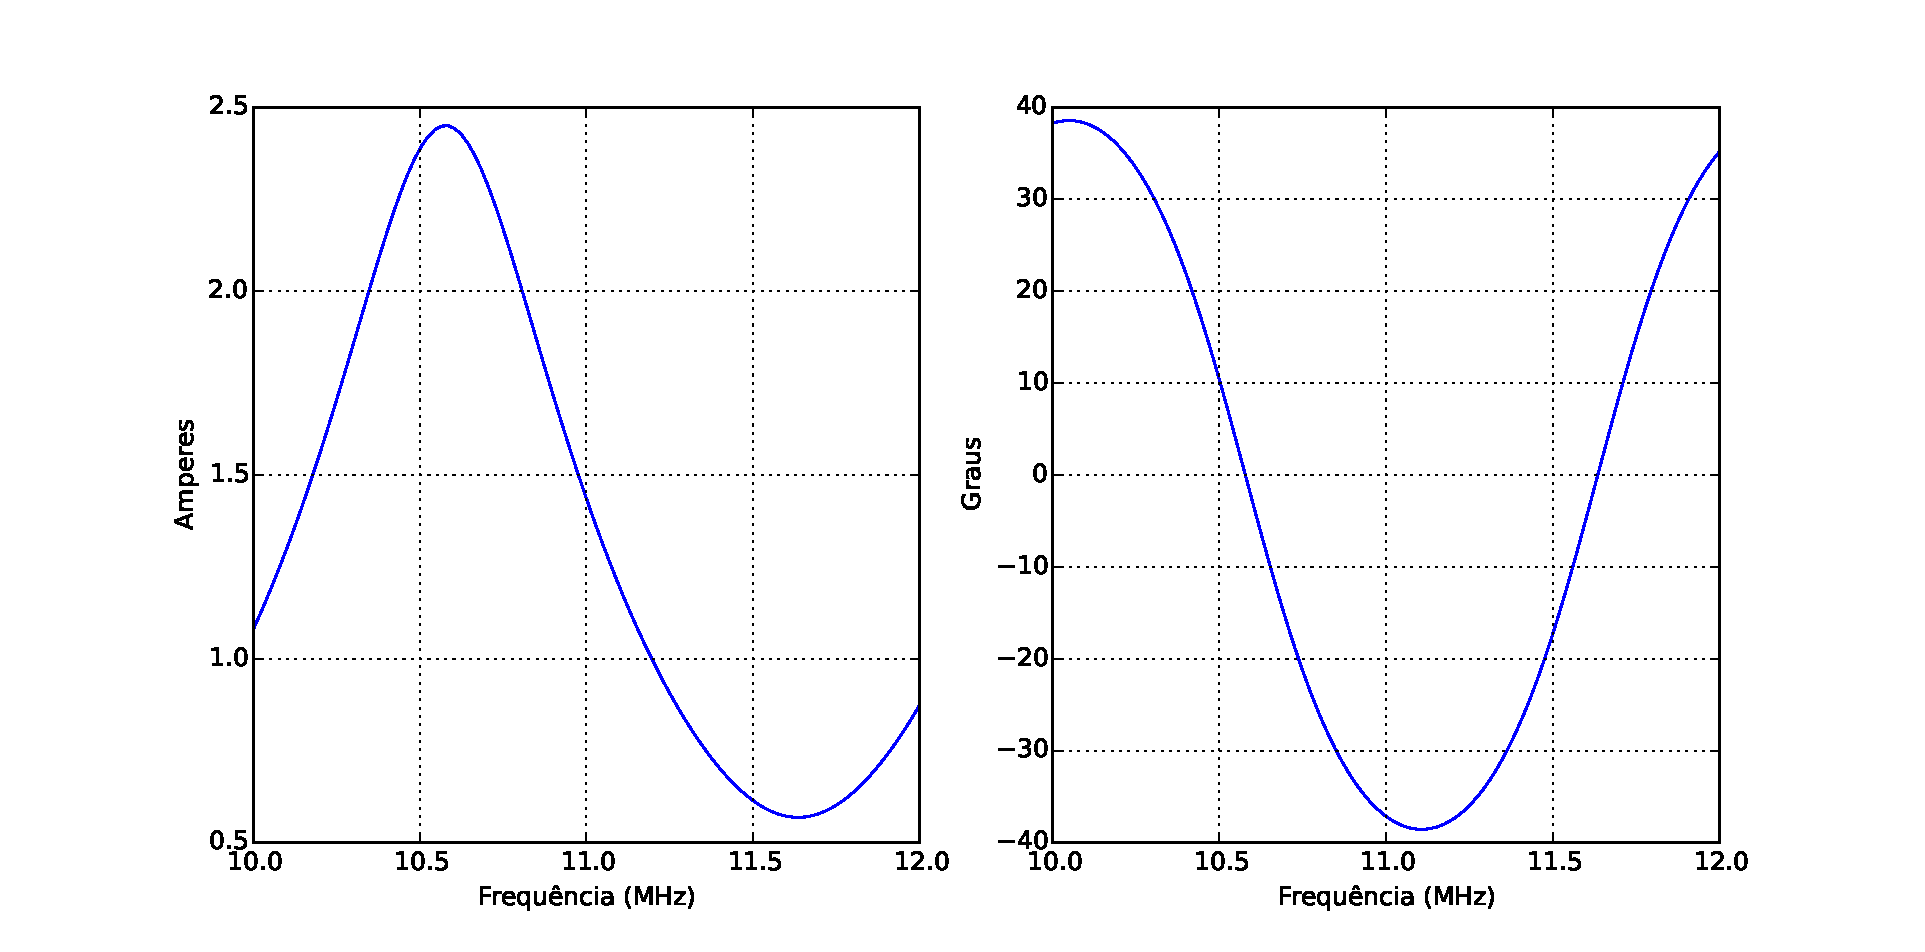
\includegraphics[scale=.5]{figures/plot_current_in.eps}
  \label{fig:Iin}
}
\subfigure[Corrente sobre a Carga]{%
  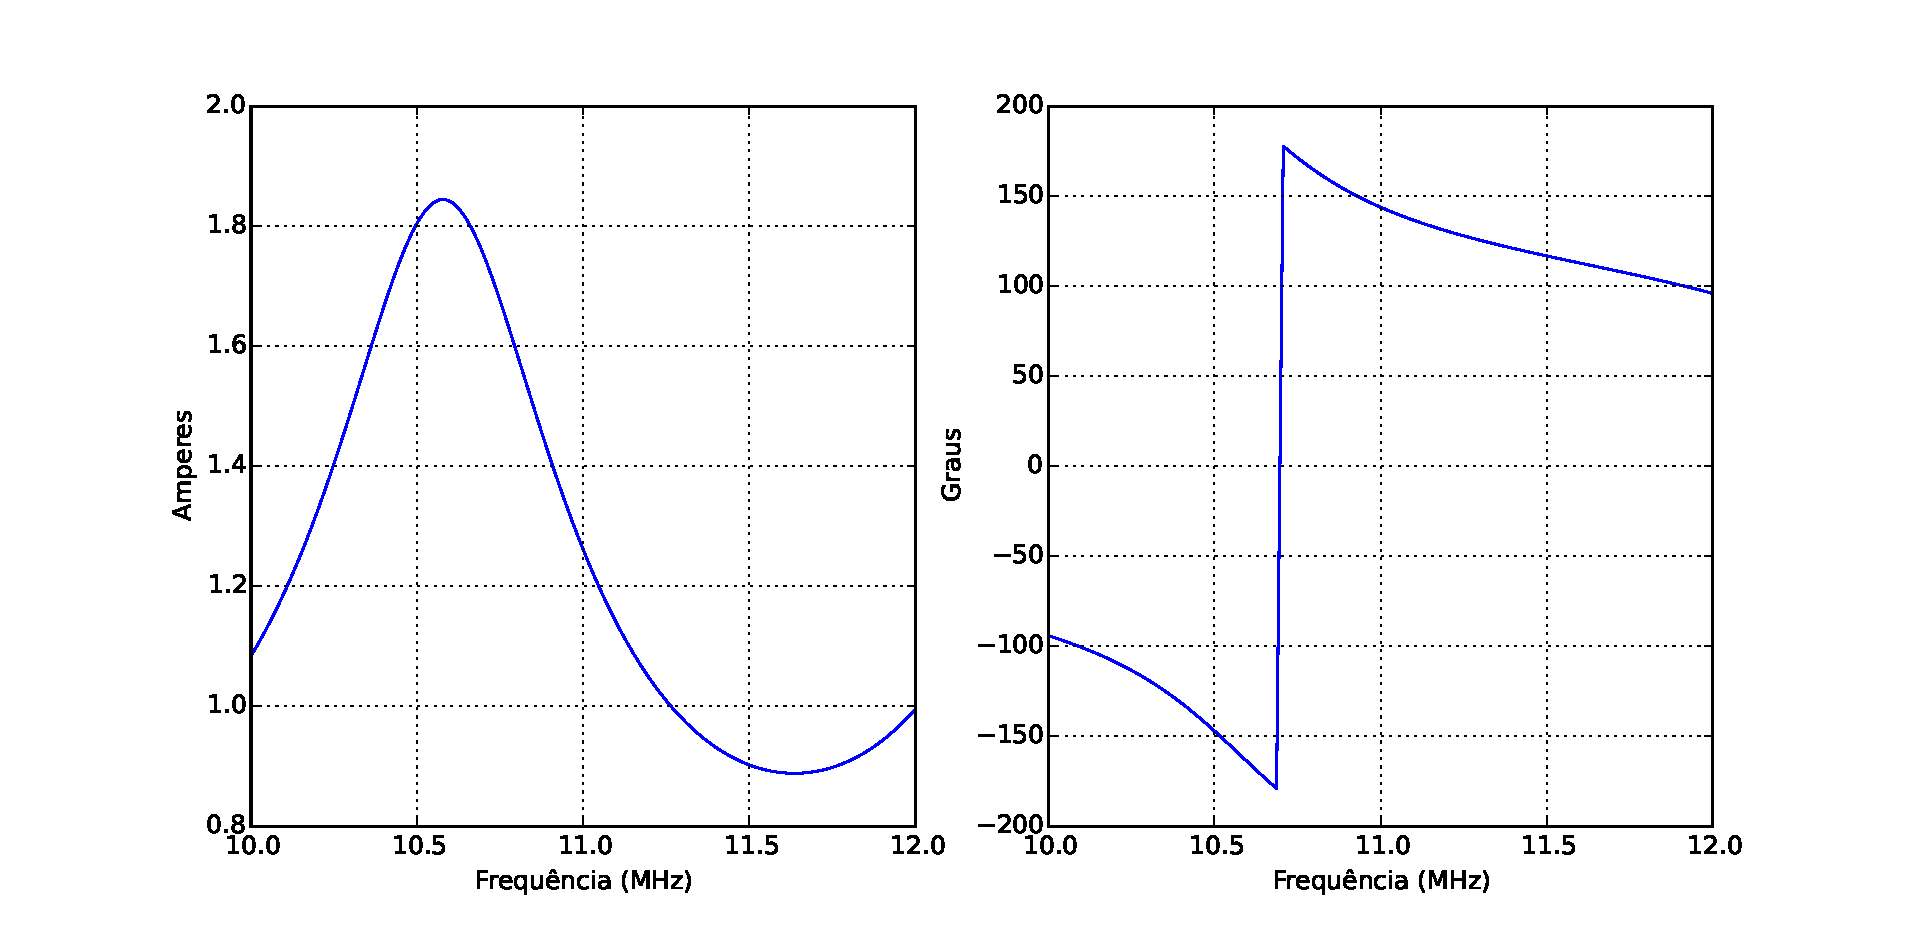
\includegraphics[scale=.5]{figures/plot_current_load.eps}
  \label{fig:Il}
}
\caption{Gráficos da amplitude e fase das Correntes na entrada e sobre carga}
\label{fig:IQ1}
\end{figure}


\end{enumerate}
% LocalWords:  Smith pt max LT LC LG RC

}
%
%\bibliographystyle{ieeetr}
%\bibliography{refpld}
%\addcontentsline{toc}{section}{Referências Bibliográficas}
%
\end{document}

%%% Local Variables:
%%% mode: latex
%%% TeX-master: t
%%% End: 
